%%%%%%%%%%%%%%%%%%%%%%%%%%%%%%%%%%%%%%%%%
% Beamer Presentation
% LaTeX Template
% Version 1.0 (10/11/12)
%
% This template has been downloaded from:
% http://www.LaTeXTemplates.com
%
% License:
% CC BY-NC-SA 3.0 (http://creativecommons.org/licenses/by-nc-sa/3.0/)
%
% Modified by Nicholas J. Gotelli
% 9 January 2021
%%%%%%%%%%%%%%%%%%%%%%%%%%%%%%%%%%%%%%%
\documentclass[12pt]{beamer}\usepackage[]{graphicx}\usepackage[]{color}
% maxwidth is the original width if it is less than linewidth
% otherwise use linewidth (to make sure the graphics do not exceed the margin)
\makeatletter
\def\maxwidth{ %
  \ifdim\Gin@nat@width>\linewidth
    \linewidth
  \else
    \Gin@nat@width
  \fi
}
\makeatother

\definecolor{fgcolor}{rgb}{0.345, 0.345, 0.345}
\newcommand{\hlnum}[1]{\textcolor[rgb]{0.686,0.059,0.569}{#1}}%
\newcommand{\hlstr}[1]{\textcolor[rgb]{0.192,0.494,0.8}{#1}}%
\newcommand{\hlcom}[1]{\textcolor[rgb]{0.678,0.584,0.686}{\textit{#1}}}%
\newcommand{\hlopt}[1]{\textcolor[rgb]{0,0,0}{#1}}%
\newcommand{\hlstd}[1]{\textcolor[rgb]{0.345,0.345,0.345}{#1}}%
\newcommand{\hlkwa}[1]{\textcolor[rgb]{0.161,0.373,0.58}{\textbf{#1}}}%
\newcommand{\hlkwb}[1]{\textcolor[rgb]{0.69,0.353,0.396}{#1}}%
\newcommand{\hlkwc}[1]{\textcolor[rgb]{0.333,0.667,0.333}{#1}}%
\newcommand{\hlkwd}[1]{\textcolor[rgb]{0.737,0.353,0.396}{\textbf{#1}}}%
\let\hlipl\hlkwb

\usepackage{framed}
\makeatletter
\newenvironment{kframe}{%
 \def\at@end@of@kframe{}%
 \ifinner\ifhmode%
  \def\at@end@of@kframe{\end{minipage}}%
  \begin{minipage}{\columnwidth}%
 \fi\fi%
 \def\FrameCommand##1{\hskip\@totalleftmargin \hskip-\fboxsep
 \colorbox{shadecolor}{##1}\hskip-\fboxsep
     % There is no \\@totalrightmargin, so:
     \hskip-\linewidth \hskip-\@totalleftmargin \hskip\columnwidth}%
 \MakeFramed {\advance\hsize-\width
   \@totalleftmargin\z@ \linewidth\hsize
   \@setminipage}}%
 {\par\unskip\endMakeFramed%
 \at@end@of@kframe}
\makeatother

\definecolor{shadecolor}{rgb}{.97, .97, .97}
\definecolor{messagecolor}{rgb}{0, 0, 0}
\definecolor{warningcolor}{rgb}{1, 0, 1}
\definecolor{errorcolor}{rgb}{1, 0, 0}
\newenvironment{knitrout}{}{} % an empty environment to be redefined in TeX

\usepackage{alltt}
% only 10,11, or 12 pt fonts
% PACKAGES-----------------------------------
\usepackage{graphicx} % Allows including images
\usepackage{booktabs} % Allows the use of \toprule, \midrule and \bottomrule in tables

% THEMES AND COLORS-------------------------
\mode<presentation> {
\usefonttheme{structurebold}
% FONTTHEMES: default, structurebold, structuresmallcapsserif, structureitalicserif, serif, professionalfonts


\usetheme{Berkeley}
% THEMES: default, AnnArbor, Antibes, Bergen, Berkeley, Berlin, Boadilla, boxes, CambridgeUS, Copenhagen, Darmstadt, Dresden, Frankfurt, Goettingen, Hannover, Ilmenau, JuanLesPins, Luebeck, Madrid, Malmoe, Marburg, Montpellier, PaloAlto, Pittsburgh, Rochester, Singapore, Szeged, Warsaw

\usecolortheme{albatross}
%COLORTHEMES: default, albatross, beaver, beetle, crane, dolphin, dove, fly, lily, orchid, rose, seagull, seahorse, sidebartab, structure, whale, wolverine 

% DISPLAY OPTIONS--------------------------
%\setbeamertemplate{footline} % To remove the footer line in all slides, uncomment this line

%\setbeamertemplate{footline}[page number] % To replace the footer line in all slides with a simple slide count, uncomment this line

%\setbeamertemplate{navigation symbols}{} % To remove the navigation symbols from the bottom of all slides, uncomment this line
}
% -----------------------------------------

% TITLE PAGE DATA--------------------------
\title[Blueberry Project]{Understanding The Fungal Microbiome in Blueberry Roots} % The short title appears at the bottom of every slide, the full title is only on the title page

\author{Sandra Nnadi} % Your name

\institute[UVM] % Your institution as it will appear on the bottom of every slide, may be shorthand to save space
{
University of Vermont \\ % Your institution for the title page
Department of Plant Biology \\
Burlington, VT 05401 USA \\ 
\medskip
\textit{sandra.nnadi@uvm.edu} % Your email address
}
\date{3 March 2021} % Date, can be changed to a custom date or \today
% -----------------------------------------

% BEGIN DOCUMENT---------------------------
\IfFileExists{upquote.sty}{\usepackage{upquote}}{}
\begin{document}

% OPTIONAL TITLE PAGE SLIDE----------------
\begin{frame}
\titlepage % Print the title page as the first slide
\end{frame}

% OPTIONAL TABLE OF CONTENTS SLIDE---------

\begin{frame}
\frametitle{Overview} % Table of contents slide, comment this block out to remove it
\tableofcontents % Throughout your presentation, if you choose to use \section{} and \subsection{} commands, these will automatically be printed on this slide as an overview of your presentation
\end{frame}

% OPTIONAL SECTION HEADERS-----------------
\section{The Blueberry Plant} % Sections can be created in order to organize your presentation into discrete blocks; all sections and subsections are automatically printed in the table of contents as an overview of the talk

\subsection{Introduction} % A subsection can be created just before a set of slides with a common theme to further break down your presentation into chunks

% SLIDE (BULLET POINTS)--------------------
\begin{frame}
\frametitle{The Blueberry Plant}
\begin{itemize}
\item Northern Highbush Blueberry
\item Ericaceae family
\item grows in acidic soil
\item mycorrhizae may improve performance
\item composition of fungal community is poorly understood
\end{itemize}
\end{frame}

% SLIDE (FIGURE)-----------------------------
\begin{frame}
\frametitle{Figure}
% Uncomment the code on this slide to include your own image from the same directory as the template  file.
% \begin{figure}
   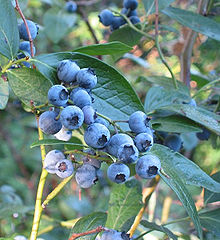
\includegraphics[width=0.5\linewidth]{220px-Vaccinium_corymbosum(01).jpg}
% use this format for absolute sizing
%\includegraphics[width=3cm, height=4cm]{filename.jpg}
% \end{figure}
\end{frame}

% SLIDE (TABLE)----------------------------
\begin{frame}
\frametitle{Table}
\begin{table}
\begin{tabular}{l l l}
\toprule
\textbf{Treatments} & \textbf{Inoculation} & \textbf{Fertilization}\\
\midrule
Control & No & No \\
Commercial Inoculum & Yes & No \\
Native Inoculum & Yes & Yes \\
\bottomrule
\end{tabular}
\caption{Experimental Design}
\end{table}
\end{frame}

%------------------------------------------------
\section{Molecular Characterization}
%------------------------------------------------
% SLIDE (PARAGRAPHS OF TEXT)---------------
\begin{frame}
\frametitle{Molecular Characterization}
A Molecular approach will be used to understand the composition of the fungal community. The Internal Transcribed Spacer {ITS} is located between the small and large subunit of the ribosomal RNA.\\~\\

The ribosomal RNA is highly conserved in all fungal species but the ITS region varies and this variation will be used to distinguish species within samples.
\end{frame}

% SLIDE (BLOCKS OF HIGHLIGHTED TEXT)-------
\begin{frame}
\frametitle{Library Preparation}
\begin{block}{1st PCR and Cleanup}
Amplify the ITS1 region with ITS forward and reverse primers then clean the PCR product with Ampure XP beads.
\end{block}

\begin{block}{2nd PCR and cleanup}
Add Index primers to adapter overhang to provide a unique identifier for each sample before pooling then clean with Ampure XP beads.
\end{block}

\begin{block}{Pooling and Sequencing}
Check quality of samples with Bioanalyzer trace, dilute final Library to 4nM then pool samples in a 2ml screw cap and submit for Illumina MiSeq Sequencing.
\end{block}

\end{frame}

% SLIDE (FINAL SLIDE)------------------------
\begin{frame}
\Huge{\centerline{The End}}
\end{frame}

%------------------------------------------------
\end{document}
